\newcommand{\datapoints}[1]{
    \begin{tikzpicture}
        \begin{axis}[
            height=3.5cm,
            width=6cm,
            xmajorticks=false,
            ymajorticks=false,
            xmin=-7,
            xmax=7,
            xlabel=\footnotesize{\textbf{x}},
            ylabel=\footnotesize{\textbf{y}}
        ]
            \addplot[
                only marks,
                blue,
                opacity=0.5,
                samples=50,
                domain=-7:7
            ] {x^3 - 3*x^2 + 2*x + 150 * rand};
            \addplot[
                red,
                domain=-7:7,
                thick
            ] {40*x-50};

            \ifnum#1>0
                \addplot[
                    green,
                    domain=-7:7,
                    thick
                ] {x^3 - 3*x^2 + 2*x};
                \node[anchor=south east, font=\tiny, align=left] (legend) at (rel axis cs: 1, 0) {
                    Linear Regression Model\\
                    Artificial Neural Network
                };
                \draw[red, thick] (rel axis cs: 0.43, 0.25) -- (rel axis cs: 0.38, 0.25);
                \draw[green, thick] (rel axis cs: 0.43, 0.11) -- (rel axis cs: 0.38, 0.11);

            \fi
        \end{axis}
    \end{tikzpicture}
}

\newcommand{\neuron}[3]{
    \node[circle, draw=black, fill=#2] (#1) at #3 {};
}

\begin{frame}{Artificial neural networks}
    \begin{tikzpicture}
        \node[] at (-5.25, -3.25) {};
        \node[] at (5.25, 3.25) {};

        \visible<1-6>{
            \node[
                draw=black,
                fill=cyan!15,
                minimum height=3cm,
                minimum width=4.3cm
            ] (model) at (0, 1) {
                \only<2-3>{$y=\beta_0+\beta_1x$}
            };
        }
        \visible<1-5>{
            \node[] (input) at ($ (model.west) + (-1, 0) $) {$\mathbf{x}$};
            \draw[-Latex] (input) -- (model);

            \node[] (output) at ($ (model.east) + (1, 0) $) {$\mathbf{y}$};
            \draw[-Latex] (model) -- (output);
        }
        \visible<1>{
            \node[font=\footnotesize] (inputlabel) at ($ (input.south) - (0, 0.5) $) {Input};
            \draw[-stealth, gray] (inputlabel) -- (input);

            \node[font=\footnotesize] (outputlabel) at ($ (output.south) - (0, 0.5) $) {Output};
            \draw[-stealth, gray] (outputlabel) -- (output);

            \node[
                anchor=south,
                font=\small
            ] at (model.north) {Predictive model};
        }
        \visible<2-3>{
            \node[
                anchor=south,
                font=\small
            ] at (model.north) {Linear regression model};
        }
        \visible<3>{
            \node[] at (-0.15, -2) {
                \datapoints{0}
            };
        }
        \visible<4-6>{
            \node[
                anchor=south,
                font=\small
            ] at (model.north) {Artificial neural network};

            \def\hsep{0.7}
            \def\vsep{0.5}
            \def\edgecolor{gray}
            \def\edgeopacity{0.5}
            \def\neuroncolour{gray}

            \neuron{n00}{\neuroncolour}{($ (model) + (-2 * \hsep, -2 * \vsep) $)}
            \neuron{n01}{\neuroncolour}{($ (model) + (-2 * \hsep, -\vsep) $)}
            \neuron{n02}{\neuroncolour}{($ (model) + (-2 * \hsep, 0) $)}
            \neuron{n03}{\neuroncolour}{($ (model) + (-2 * \hsep, \vsep) $)}
            \neuron{n04}{\neuroncolour}{($ (model) + (-2 * \hsep, 2 * \vsep) $)}

            \neuron{n10}{\neuroncolour}{($ (model) + (-\hsep, -1.5 * \vsep) $)}
            \neuron{n11}{\neuroncolour}{($ (model) + (-\hsep, -0.5 * \vsep) $)}
            \neuron{n12}{\neuroncolour}{($ (model) + (-\hsep, 0.5 * \vsep) $)}
            \neuron{n13}{\neuroncolour}{($ (model) + (-\hsep, 1.5 * \vsep) $)}

            \neuron{n20}{\neuroncolour}{($ (model) + (0, -\vsep) $)}
            \neuron{n21}{\neuroncolour}{(model)}
            \neuron{n22}{\neuroncolour}{($ (model) + (0, \vsep) $)}

            \neuron{n30}{\neuroncolour}{($ (model) + (\hsep, -0.5 * \vsep) $)}
            \neuron{n31}{\neuroncolour}{($ (model) + (\hsep, 0.5 * \vsep) $)}

            \neuron{n40}{\neuroncolour}{($ (model) + (2 * \hsep, 0) $)}

            \draw[-stealth, \edgecolor, opacity=\edgeopacity] (model.west) -- (n00);
            \draw[-stealth, \edgecolor, opacity=\edgeopacity] (model.west) -- (n01);
            \draw[-stealth, \edgecolor, opacity=\edgeopacity] (model.west) -- (n02);
            \draw[-stealth, \edgecolor, opacity=\edgeopacity] (model.west) -- (n03);
            \draw[-stealth, \edgecolor, opacity=\edgeopacity] (model.west) -- (n04);

            \foreach \i in {0,...,4} {
                \foreach \j in {0,...,3} {
                    \draw[\edgecolor, opacity=\edgeopacity] (n0\i) -- (n1\j);
                }
            }
            \foreach \i in {0,...,3} {
                \foreach \j in {0,...,2} {
                    \draw[\edgecolor, opacity=\edgeopacity] (n1\i) -- (n2\j);
                }
            }
            \foreach \i in {0,...,2} {
                \foreach \j in {0,...,1} {
                    \draw[\edgecolor, opacity=\edgeopacity] (n2\i) -- (n3\j);
                }
            }
            \foreach \i in {0,...,1} {
                \draw[\edgecolor, opacity=\edgeopacity] (n3\i) -- (n40);
            }

            \draw[-stealth, \edgecolor, opacity=\edgeopacity] (n40) -- (model.east);
        }
        \visible<5>{
            \node[] at (-0.15, -2) {
                \datapoints{1}
            };
        }
        \visible<6>{
            \node[anchor=east, draw=black, inner sep=0pt, outer sep=3pt] (input) at ($ (model.west) + (-0.77, 0) $) {
                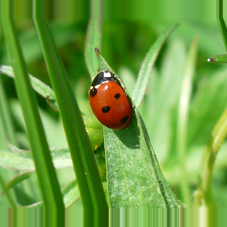
\includegraphics[width=2cm]{data/ladybug.png}
            };
            \draw[-Latex] (input) -- (model);

            \node[anchor=west] (output) at ($ (model.east) + (0.77, 0) $) {
                Ladybug
            };
            \draw[-Latex] (model) -- (output);
        }
    \end{tikzpicture}
\end{frame}

\begin{frame}{Artificial neural networks: Interpretability}
    \begin{tikzpicture}
        \node[] at (-5.25, -3.25) {};
        \node[] at (5.25, 3.25) {};

        \node[
            draw=black,
            fill=cyan!15,
            minimum height=3cm,
            minimum width=4.3cm
        ] (model) at (0, 1) {};
        \node[
            anchor=south,
            font=\small
        ] at (model.north) {Artificial neural network};

        \visible<1-4>{
            \node[] (input) at ($ (model.west) + (-1, 0) $) {$\mathbf{x}$};
            \draw[-Latex] (input) -- (model);
        }
        \visible<1-10>{
            \node[] (output) at ($ (model.east) + (1, 0) $) {$\mathbf{y}$};
            \draw[-Latex] (model) -- (output);
        }
        \visible<1,3->{
            \node[
                anchor=south,
                font=\small
            ] at (model.north) {Artificial neural network};

            \def\hsep{0.7}
            \def\vsep{0.5}
            \def\edgecolor{gray}
            \def\edgeopacity{0.5}
            \def\neuroncolour{gray}

            \visible<1-5>{
                \neuron{n00}{\neuroncolour}{($ (model) + (-2 * \hsep, -2 * \vsep) $)}
                \neuron{n01}{\neuroncolour}{($ (model) + (-2 * \hsep, -\vsep) $)}
                \neuron{n02}{\neuroncolour}{($ (model) + (-2 * \hsep, 0) $)}
                \neuron{n03}{\neuroncolour}{($ (model) + (-2 * \hsep, \vsep) $)}
                \neuron{n04}{\neuroncolour}{($ (model) + (-2 * \hsep, 2 * \vsep) $)}
            }
            \visible<6->{
                \neuron{n00}{black!25}{($ (model) + (-2 * \hsep, -2 * \vsep) $)}
                \neuron{n01}{black!90}{($ (model) + (-2 * \hsep, -\vsep) $)}
                \neuron{n02}{black!72}{($ (model) + (-2 * \hsep, 0) $)}
                \neuron{n03}{black!99}{($ (model) + (-2 * \hsep, \vsep) $)}
                \neuron{n04}{black!10}{($ (model) + (-2 * \hsep, 2 * \vsep) $)}
            }

            \visible<1-6>{
                \neuron{n10}{\neuroncolour}{($ (model) + (-\hsep, -1.5 * \vsep) $)}
                \neuron{n11}{\neuroncolour}{($ (model) + (-\hsep, -0.5 * \vsep) $)}
                \neuron{n12}{\neuroncolour}{($ (model) + (-\hsep, 0.5 * \vsep) $)}
                \neuron{n13}{\neuroncolour}{($ (model) + (-\hsep, 1.5 * \vsep) $)}
            }
            \visible<7->{
                \neuron{n10}{black!55}{($ (model) + (-\hsep, -1.5 * \vsep) $)}
                \neuron{n11}{black!92}{($ (model) + (-\hsep, -0.5 * \vsep) $)}
                \neuron{n12}{black!31}{($ (model) + (-\hsep, 0.5 * \vsep) $)}
                \neuron{n13}{black!7}{($ (model) + (-\hsep, 1.5 * \vsep) $)}
            }
            \visible<1-7>{
                \neuron{n20}{\neuroncolour}{($ (model) + (0, -\vsep) $)}
                \neuron{n21}{\neuroncolour}{(model)}
                \neuron{n22}{\neuroncolour}{($ (model) + (0, \vsep) $)}
            }
            \visible<8->{
                \neuron{n20}{black!50}{($ (model) + (0, -\vsep) $)}
                \neuron{n21}{black!10}{(model)}
                \neuron{n22}{black!100}{($ (model) + (0, \vsep) $)}
            }

            \visible<1-8>{
                \neuron{n30}{\neuroncolour}{($ (model) + (\hsep, -0.5 * \vsep) $)}
                \neuron{n31}{\neuroncolour}{($ (model) + (\hsep, 0.5 * \vsep) $)}
            }
            \visible<9->{
                \neuron{n30}{black!75}{($ (model) + (\hsep, -0.5 * \vsep) $)}
                \neuron{n31}{black!65}{($ (model) + (\hsep, 0.5 * \vsep) $)}
            }
            \visible<1-9>{
                \neuron{n40}{\neuroncolour}{($ (model) + (2 * \hsep, 0) $)}
            }
            \visible<10->{
                \neuron{n40}{black!95}{($ (model) + (2 * \hsep, 0) $)}
            }

            \visible<1-5,7->{
                \draw[-stealth, \edgecolor, opacity=\edgeopacity] (model.west) -- (n00);
                \draw[-stealth, \edgecolor, opacity=\edgeopacity] (model.west) -- (n01);
                \draw[-stealth, \edgecolor, opacity=\edgeopacity] (model.west) -- (n02);
                \draw[-stealth, \edgecolor, opacity=\edgeopacity] (model.west) -- (n03);
                \draw[-stealth, \edgecolor, opacity=\edgeopacity] (model.west) -- (n04);
            }
            \visible<6>{
                \draw[-stealth, red, opacity=\edgeopacity] (model.west) -- (n00);
                \draw[-stealth, red, opacity=\edgeopacity] (model.west) -- (n01);
                \draw[-stealth, red, opacity=\edgeopacity] (model.west) -- (n02);
                \draw[-stealth, red, opacity=\edgeopacity] (model.west) -- (n03);
                \draw[-stealth, red, opacity=\edgeopacity] (model.west) -- (n04);
            }

            \visible<1-6,8->{
                \foreach \i in {0,...,4} {
                    \foreach \j in {0,...,3} {
                        \draw[\edgecolor, opacity=\edgeopacity] (n0\i) -- (n1\j);
                    }
                }
            }
            \visible<7>{
                \foreach \i in {0,...,4} {
                    \foreach \j in {0,...,3} {
                        \draw[red, opacity=\edgeopacity] (n0\i) -- (n1\j);
                    }
                }
            }

            \visible<1-7,9->{
                \foreach \i in {0,...,3} {
                    \foreach \j in {0,...,2} {
                        \draw[\edgecolor, opacity=\edgeopacity] (n1\i) -- (n2\j);
                    }
                }
            }
            \visible<8>{
                \foreach \i in {0,...,3} {
                    \foreach \j in {0,...,2} {
                        \draw[red, opacity=\edgeopacity] (n1\i) -- (n2\j);
                    }
                }
            }

            \visible<1-8,10->{
                \foreach \i in {0,...,2} {
                    \foreach \j in {0,...,1} {
                        \draw[\edgecolor, opacity=\edgeopacity] (n2\i) -- (n3\j);
                    }
                }
            }
            \visible<9>{
                \foreach \i in {0,...,2} {
                    \foreach \j in {0,...,1} {
                        \draw[red, opacity=\edgeopacity] (n2\i) -- (n3\j);
                    }
                }
            }
            \visible<1-9,11->{
                \foreach \i in {0,...,1} {
                    \draw[\edgecolor, opacity=\edgeopacity] (n3\i) -- (n40);
                }
            }
            \visible<10>{
                \foreach \i in {0,...,1} {
                    \draw[red, opacity=\edgeopacity] (n3\i) -- (n40);
                }
            }

            \visible<1-10,12-13>{
                \draw[-stealth, \edgecolor, opacity=\edgeopacity] (n40) -- (model.east);
            }
            \visible<11>{
                \draw[-stealth, red, opacity=\edgeopacity] (n40) -- (model.east);
            }
        }
        \visible<2>{
            \node[
                draw=black,
                fill=black,
                minimum height=3cm,
                minimum width=4.3cm
            ] (model) at (0, 1) {};
        }
        \visible<3>{
            \node[] at (-0.15, -2) {
                \datapoints{1}
            };
        }
        \visible<5-11>{
            \node[] (input) at ($ (model.west) + (-1, 0) $) {$5$};
        }
        \visible<5,7-11>{
            \draw[-Latex] (input) -- (model);
        }
        \visible<6>{
            \draw[-Latex, red] (input) -- (model);
        }
        \visible<11>{
            \node[text=red] (output) at ($ (model.east) + (1, 0) $) {3};
            \draw[-Latex, red] (model) -- (output);
        }
        \visible<12-13>{
            \node[anchor=east, draw=black, inner sep=0pt, outer sep=3pt] (input) at ($ (model.west) + (-0.77, 0) $) {
                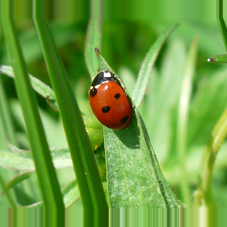
\includegraphics[width=2cm]{data/ladybug.png}
            };
            \draw[-Latex] (input) -- (model);

            \node[anchor=west] (output) at ($ (model.east) + (0.77, 0) $) {
                Ladybug
            };
            \draw[-Latex] (model) -- (output);
        }
        \visible<6-13>{
            \node[] at (0, -2.5) {
                $n^i_j = f(\sum\limits_{k=0}^n w^{i}_{jk} n^{i-1}_k)$
            };
        }
        \visible<13>{
            \node[anchor=north] (pass) at (model.south) {
                \textbf{\textit{Forward pass}}
            };
            \draw[-stealth] (pass.south west) -- (pass.south east);
        }
    \end{tikzpicture}
\end{frame}

\begin{frame}{Artificial neural networks: Explainability}
        \begin{tikzpicture}
            \node[draw=black] at (-5.25, -3.25) {};
            \node[draw=black] at (5.25, 3.25) {};
            \visible<1-8>{
                \node[
                    draw=black,
                    fill=cyan!15,
                    minimum height=3cm,
                    minimum width=4.3cm
                ] (model) at (0, 1) {};
                \node[
                    anchor=south,
                    font=\small
                ] at (model.north) {Artificial neural network};

                \def\hsep{0.7}
                \def\vsep{0.5}
                \def\edgecolor{gray}
                \def\edgeopacity{0.5}
                \def\neuroncolour{gray}

                \visible<1-6>{
                    \neuron{n00}{black!25}{($ (model) + (-2 * \hsep, -2 * \vsep) $)}
                    \neuron{n01}{black!90}{($ (model) + (-2 * \hsep, -\vsep) $)}
                    \neuron{n02}{black!72}{($ (model) + (-2 * \hsep, 0) $)}
                    \neuron{n03}{black!99}{($ (model) + (-2 * \hsep, \vsep) $)}
                    \neuron{n04}{black!10}{($ (model) + (-2 * \hsep, 2 * \vsep) $)}
                }
                \visible<7->{
                    \neuron{n00}{red!25!black}{($ (model) + (-2 * \hsep, -2 * \vsep) $)}
                    \neuron{n01}{red!90!black}{($ (model) + (-2 * \hsep, -\vsep) $)}
                    \neuron{n02}{yellow!15!red}{($ (model) + (-2 * \hsep, 0) $)}
                    \neuron{n03}{red!99!black}{($ (model) + (-2 * \hsep, \vsep) $)}
                    \neuron{n04}{red!10!black}{($ (model) + (-2 * \hsep, 2 * \vsep) $)}
                }
                \visible<1-5>{
                    \neuron{n10}{black!55}{($ (model) + (-\hsep, -1.5 * \vsep) $)}
                    \neuron{n11}{black!92}{($ (model) + (-\hsep, -0.5 * \vsep) $)}
                    \neuron{n12}{black!31}{($ (model) + (-\hsep, 0.5 * \vsep) $)}
                    \neuron{n13}{black!7}{($ (model) + (-\hsep, 1.5 * \vsep) $)}
                }
                \visible<6->{
                    \neuron{n10}{red!55!black}{($ (model) + (-\hsep, -1.5 * \vsep) $)}
                    \neuron{n11}{yellow!20!red}{($ (model) + (-\hsep, -0.5 * \vsep) $)}
                    \neuron{n12}{yellow!90!red}{($ (model) + (-\hsep, 0.5 * \vsep) $)}
                    \neuron{n13}{red!7!black}{($ (model) + (-\hsep, 1.5 * \vsep) $)}
                }

                \visible<1-4>{
                    \neuron{n20}{black!50}{($ (model) + (0, -\vsep) $)}
                    \neuron{n21}{black!10}{(model)}
                    \neuron{n22}{black!100}{($ (model) + (0, \vsep) $)}
                }
                \visible<5->{
                    \neuron{n20}{red!90!black}{($ (model) + (0, -\vsep) $)}
                    \neuron{n21}{red!30!black}{(model)}
                    \neuron{n22}{yellow!70!red}{($ (model) + (0, \vsep) $)}
                }

                \visible<1-3>{
                    \neuron{n30}{black!75}{($ (model) + (\hsep, -0.5 * \vsep) $)}
                    \neuron{n31}{black!65}{($ (model) + (\hsep, 0.5 * \vsep) $)}
                }
                \visible<4->{
                    \neuron{n30}{yellow!40!red}{($ (model) + (\hsep, -0.5 * \vsep) $)}
                    \neuron{n31}{red!65!black}{($ (model) + (\hsep, 0.5 * \vsep) $)}
                }

                \visible<1-2>{
                    \neuron{n40}{black!95}{($ (model) + (2 * \hsep, 0) $)}
                }
                \visible<3->{
                    \neuron{n40}{red}{($ (model) + (2 * \hsep, 0) $)}
                }

                \visible<1-7>{
                    \draw[-stealth, \edgecolor, opacity=\edgeopacity] (model.west) -- (n00);
                    \draw[-stealth, \edgecolor, opacity=\edgeopacity] (model.west) -- (n01);
                    \draw[-stealth, \edgecolor, opacity=\edgeopacity] (model.west) -- (n02);
                    \draw[-stealth, \edgecolor, opacity=\edgeopacity] (model.west) -- (n03);
                    \draw[-stealth, \edgecolor, opacity=\edgeopacity] (model.west) -- (n04);
                }
                \visible<8>{
                    \draw[stealth-, red, opacity=\edgeopacity] (model.west) -- (n00);
                    \draw[stealth-, red, opacity=\edgeopacity] (model.west) -- (n01);
                    \draw[stealth-, red, opacity=\edgeopacity] (model.west) -- (n02);
                    \draw[stealth-, red, opacity=\edgeopacity] (model.west) -- (n03);
                    \draw[stealth-, red, opacity=\edgeopacity] (model.west) -- (n04);
                }

                \visible<1-6,7->{
                    \foreach \i in {0,...,4} {
                        \foreach \j in {0,...,3} {
                            \draw[\edgecolor, opacity=\edgeopacity] (n0\i) -- (n1\j);
                        }
                    }
                }
                \visible<7>{
                    \foreach \i in {0,...,4} {
                        \foreach \j in {0,...,3} {
                            \draw[stealth-, red, opacity=\edgeopacity] (n0\i) -- (n1\j);
                        }
                    }
                }

                \visible<1-5,6->{
                    \foreach \i in {0,...,3} {
                        \foreach \j in {0,...,2} {
                            \draw[\edgecolor, opacity=\edgeopacity] (n1\i) -- (n2\j);
                        }
                    }
                }
                \visible<6>{
                    \foreach \i in {0,...,3} {
                        \foreach \j in {0,...,2} {
                            \draw[stealth-, red, opacity=\edgeopacity] (n1\i) -- (n2\j);
                        }
                    }
                }

                \visible<1-4,6->{
                    \foreach \i in {0,...,2} {
                        \foreach \j in {0,...,1} {
                            \draw[\edgecolor, opacity=\edgeopacity] (n2\i) -- (n3\j);
                        }
                    }
                }
                \visible<5>{
                    \foreach \i in {0,...,2} {
                        \foreach \j in {0,...,1} {
                            \draw[stealth-, red, opacity=\edgeopacity] (n2\i) -- (n3\j);
                        }
                    }

                }

                \visible<1-3,5->{
                    \foreach \i in {0,...,1} {
                        \draw[\edgecolor, opacity=\edgeopacity] (n3\i) -- (n40);
                    }
                }
                \visible<4>{
                    \foreach \i in {0,...,1} {
                        \draw[stealth-, red, opacity=\edgeopacity] (n3\i) -- (n40);
                    }
                }

                \visible<1-2>{
                    \draw[-stealth, \edgecolor, opacity=\edgeopacity] (n40) -- (model.east);
                }
                \visible<3->{
                    \draw[stealth-, red, opacity=\edgeopacity] (n40) -- (model.east);
                }

                \visible<1>{
                    \node[anchor=north] (pass) at (model.south) {
                        \textbf{\textit{Forward pass}}
                    };
                    \draw[-stealth] (pass.south west) -- (pass.south east);

                    \node[] at (0, -2.5) {
                        $n^i_j = f(\sum\limits_{k=0}^n w^{i}_{jk} n^{i-1}_k)$
                    };
                }
                \visible<1-7>{
                    \node[anchor=east, draw=black, inner sep=0pt, outer sep=3pt] (input) at ($ (model.west) + (-0.77, 0) $) {
                        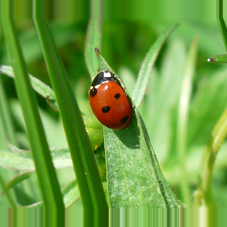
\includegraphics[width=2cm]{data/ladybug.png}
                    };
                    \draw[-Latex] (input) -- (model);
                }
                \visible<1-2>{
                    \node[anchor=west] (output) at ($ (model.east) + (0.77, 0) $) {
                        Ladybug
                    };
                    \draw[-Latex] (model) -- (output);
                }
                \visible<2->{
                    \node[anchor=north, text=red] (pass) at (model.south) {
                        \textbf{\textit{Backward pass}}
                    };
                    \draw[stealth-, red] (pass.south west) -- (pass.south east);

                    \node[] at (0, -2.3) {
                        $R^{i-1}_j=\sum\limits_{k} \dfrac{n^{(i-1)}_jw^{(i-1)}_{jk}}{\sum\limits_{l} n^{(i-1)}_lw^{(i-1)}_{lk}}R^i_k$
                    };
                }
                \visible<3->{
                    \node[anchor=west, text=red] (output) at ($ (model.east) + (0.77, 0) $) {
                        Ladybug
                    };
                    \draw[Latex-,red] (model) -- (output);
                }
                \visible<8>{
                    \node[anchor=east, draw=black, inner sep=0pt, outer sep=3pt] (input) at ($ (model.west) + (-0.77, 0) $) {
                        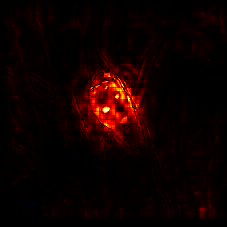
\includegraphics[width=2cm]{data/ladybug_explanation.png}
                    };
                    \draw[Latex-,red] (input) -- (model);
                }
            }
            \visible<9-11>{
                \node[text width=10cm] at (0, 0) {
                    \textbf{Reasons to use explainable AI:}
                    \begin{itemize}
                        \item Sanity check models
                        \item Building trust among users
                        \item<10-> Scientific discovery
                        \item<11> Characterize heterogeneity in groups we consider (somewhat) homogeneous
                    \end{itemize}
                };
            }
        \end{tikzpicture}
\end{frame}

\begin{frame}{Explainable AI: The central idea}
    \def\imagesize{1.5cm}

    \begin{tikzpicture}
        \node[] at (-5.25, -3.5) {};
        \node[] at (5.25, 3.5) {};

        \node[anchor=north west, draw=black, inner sep=0pt] (cat) at (-3.75, 2.9) {
            
\includegraphics[width=\imagesize]{data/cat.png}
        };
        \node[anchor=north west, draw=black, inner sep=0pt] (rooster) at ($ (cat.north east) + (0.5, 0) $) {
            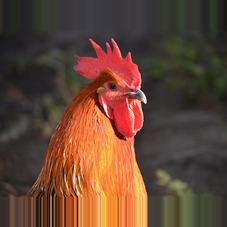
\includegraphics[width=\imagesize]{data/rooster.png}
        };
        \node[anchor=north west, draw=black, inner sep=0pt] (rooster2) at ($ (rooster.north east) + (0.5, 0) $) {
            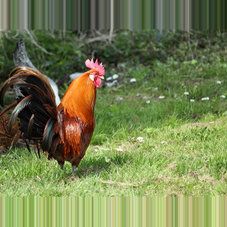
\includegraphics[width=\imagesize]{data/rooster2.png}
        };
        \node[anchor=north west, draw=black, inner sep=0pt] (rabbit) at ($ (rooster2.north east) + (0.5, 0) $) {
            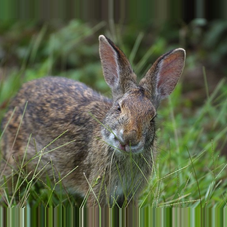
\includegraphics[width=\imagesize]{data/rabbit.png}
        };

        \draw[dashed] ($ (cat.north west) + (-0.1, 0.1) $) --
                    ($ (rabbit.north east) + (0.1, 0.1) $) --
                 ($ (rabbit.south east) + (0.1, -0.1) $) --
                 ($ (cat.south west) + (-0.1, -0.1) $) -- cycle;
        \node[anchor=south] at ($ (cat.north west)!0.5!(rabbit.north east) + (0, 0.1) $) {
            Animals
        };
        \visible<2->{
            \node[anchor=west, draw=black, fill=black!80, rounded corners=0.1cm, text=white, align=center] (supervised) at (-5, -0.3) {
                Supervised\\learning
            };

            \draw[-stealth, line width=3pt, draw=gray] ($ (cat.south west)!0.5!(rabbit.south east) + (-0.1, -0.1) $) |- ($ (supervised.north) + (0, 0.5) $) -- (supervised.north);
        }
        \visible<2-3>{
            \node[] (animals) at ($ (supervised) - (0, 1.5) $) {
                Animals
            };
            \draw[-stealth, line width=3pt, draw=gray] (supervised) -- (animals);
        }
        \visible<3->{
            \node[anchor=east, draw=black, fill=black!80, rounded corners=0.1cm, text=white, align=center] (unsupervised) at (4.2, -0.3) {
                Unsupervised\\learning
            };
        }
        \visible<3>{
            \draw[-stealth, line width=3pt, draw=gray] ($ (cat.south west)!0.5!(rabbit.south east) + (0.05, -0.1) $) |- ($ (unsupervised.north) + (0, 0.5) $) -- (unsupervised.north);

            \node[anchor=north west, draw=black, inner sep=0pt] (uscat) at ($ (unsupervised.south) + (0.2, -0.5) $)  {
                
\includegraphics[width=1cm]{data/cat.png}
            };
            \node[anchor=north, draw=black, inner sep=0pt] (usrabbit) at ($ (uscat.south) - (0, 0.1) $) {
                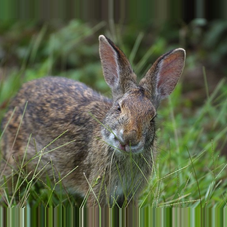
\includegraphics[width=1cm]{data/rabbit.png}
            };
            \node[anchor=west, draw=black, inner sep=0pt] (usrooster2) at ($ (uscat.east)!0.5!(usrabbit.east) + (0.1, 0) $) {
                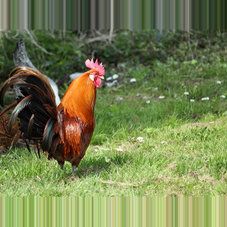
\includegraphics[width=1cm]{data/rooster2.png}
            };
            \node[anchor=north east, draw=black, inner sep=0pt] (usrooster) at ($ (unsupervised.south) + (-0.2, -1) $) {
                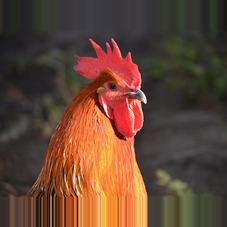
\includegraphics[width=1cm]{data/rooster.png}
            };

            \draw[densely dotted, thick] (unsupervised.south) -- ++(0, -2.7);
        }
        \visible<4->{
            \node[anchor=east, inner sep=0pt] at ($ (supervised.east)!0.5!(unsupervised.west) + (-0.05, 0) $) (catheat) {
                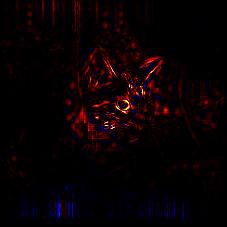
\includegraphics[width=1.5cm]{data/cat_heatmap.png}
            };
            \node[anchor=north west, inner sep=0pt] at ($ (catheat.north east) + (0.1, 0) $) (rabbitheat) {
                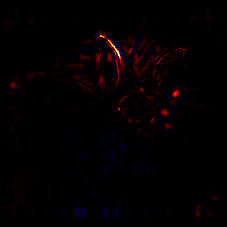
\includegraphics[width=1.5cm]{data/rabbit_explanation.png}
            };
            \node[anchor=north west, inner sep=0pt] at ($ (catheat.south west) - (0, 0.1) $) (roosterheat) {
                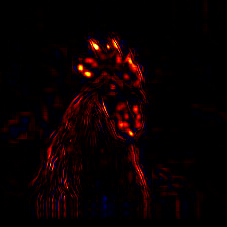
\includegraphics[width=1.5cm]{data/rooster_heatmap.png}
            };
            \node[anchor=north west, inner sep=0pt] at ($ (rabbitheat.south west) - (0, 0.1) $) (rooster2heat) {
                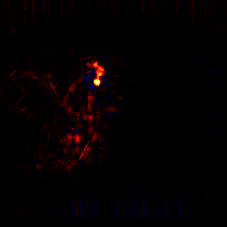
\includegraphics[width=1.5cm]{data/rooster2_heatmap.png}
            };

            \draw[-stealth, line width=3pt, draw=gray] (supervised) -- (catheat);
            \draw[-stealth, line width=3pt, draw=gray] (rabbitheat) -- (unsupervised);
        }
        \visible<5>{
            \node[draw=white, densely dotted, inner sep=0pt, minimum width=0.5cm, minimum height=0.35cm] at ($ (roosterheat) + (-0.03, 0.37) $) {};
            \node[draw=white, densely dotted, inner sep=0pt, minimum width=0.15cm, minimum height=0.15cm] at ($ (rooster2heat) + (-0.12, 0.3) $) {};
        }
    \end{tikzpicture}
\end{frame}

\begin{frame}{Explainable AI: Caveats}
    \begin{tikzpicture}
        \node[draw=black] at (-5.25, -3.25) {};
        \node[draw=black] at (5.25, 3.25) {};

        \node[
            draw=black,
            fill=cyan!15,
            minimum height=3cm,
            minimum width=4.3cm
        ] (model) at (0, 1) {};
        \node[
            anchor=south,
            font=\small
        ] at (model.north) {Predictive model};

        \node[anchor=east, draw=black, inner sep=0pt, outer sep=3pt] (input) at ($ (model.west) + (-0.77, 0) $) {
            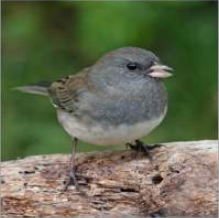
\includegraphics[width=2cm]{data/bird.png}
        };
        \draw[-Latex] (input) -- (model);

        \node[anchor=west] (output) at ($ (model.east) + (0.77, 0) $) {
            Bird
        };
        \draw[-Latex] (model) -- (output);

        \only<2-3>{
            \node[draw=black, inner sep=0pt] (explanation) at (0, -2.3) {
                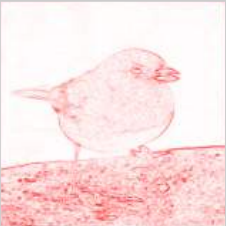
\includegraphics[width=2cm]{data/edgedetector.png}
            };
        }
        \only<2>{
            \draw[-stealth, line width=4pt, gray] (model) -- (explanation);
        }
        \only<3>{
            \draw[-stealth, line width=4pt, gray] ($ (input.south) + (0, 0.1) $) to [out=270, in=180] (explanation);
        }
    \end{tikzpicture}
\end{frame}
